\subsubsection{Processo de modelagem}
\noindent Na etapa de modelagem foi realizada a composição dos modelos genéricos utilizando ferramentas computacionais de simulação de eficiência energética. Nesta fase foram configurados e ajustados os parâmetros incorporados aos modelos, como as características volumétricas, dados de desempenho dos equipamentos e soluções arquitetônicas.\vspace*{0.3cm} \newline
\noindent Trabalhos como o de Didoné \citeyear{Didone2014}, que realizou um estudo paramétrico de estratégias para edificações com balanço energético nulo no Brasil, utilizou o \textit{EnergyPlus} como principal ferramenta para simulação dos cenários termoenergéticos propostos. Carlo \citeyear{Carlo2008}, que desenvolveu uma metodologia de avaliação da eficiência energética para a envoltória de edificações não-residenciais, também utilizou essa ferramenta por reunir funções que auxiliariam na simulação de desempenho termoenergético e de parâmetros econômicos para verificação do consumo energético do modelo proposto.\vspace*{0.3cm} \newline
\noindent Outros autores aplicam o EnergyPlus por ser um software open source ou seja, software livre, amplamente utilizado pela comunidade cientifica e por reduzir os esforços no desenvolvimento de modelos matemáticos complexos para simulação de cenários termoenergéticos, auxiliando na otimização energética dos modelos propostos em estudo \cite{Vuong2015,Dahanayake2017,Shen2018,Kamal2019}.\vspace*{0.3cm} \newline
\noindent Portanto, a escolha da ferramenta mais apropriada para a modelagem dos parâmetros escolhidos como recurso ao processo de simulação da metodologia foi necessária. Seguindo a premissa de que a ferramenta deveria ser de livre acesso, ser validada em âmbito acadêmico e apresentar o maior volume de utilização em estudos de caso possível, como exemplificado na Figura \ref{fig:figure15}, foi adotado o software de simulação de energia em edificações \textit{EnergyPlus} 9.1.0-08d2e308bb \cite{U.S.DepartmentofEnergy-USDOE2011,Athienitis2015}.\vspace*{0.3cm} \newline
\noindent Da mesma forma, segundo Brackney et al. \citeyear{Brackney2018}, para facilitar o processo de configuração volumétrica e energética dos modelos, foram utilizadas ferramentas de suporte, que forneceram a interface entre o simulador e a ferramenta de modelagem. Estas ferramentas foram o \textit{SketchUp} 2017 trial version, versão 17.0.18899 \cite{TrimbleInc.2019}, para modelagem computacional tridimensional do edifício, e as extensões open-source para \textit{SketchUp, OpenStudio} v2.8.0, e a ferramenta de análise paramétrica \textit{Parametric Analysis Tool} – PAT.\vspace*{0.3cm} \newline
\begin{figure}[H]
    \centering
    \caption{\textit{Softwares} mais utilizados em simulação de eficiência de edificações.}
    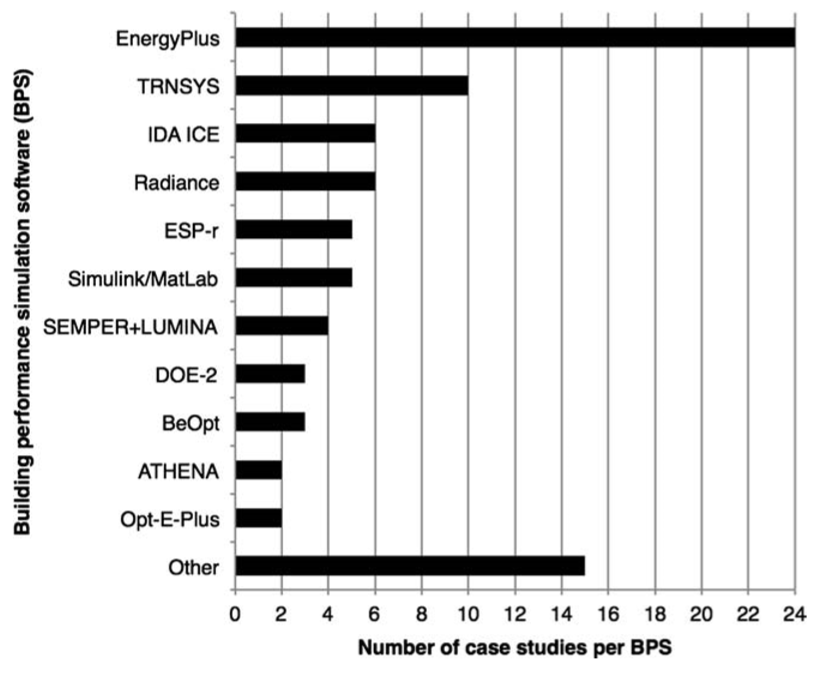
\includegraphics[width=0.8\textwidth]{figures/fig15-grafico-soft.png}
    \begin{flushleft}
        \par \small Fonte: adaptado de Athienitis; O’Brien (2015, tradução nossa).
    \end{flushleft}
    \label{fig:figure15}
\end{figure}
\noindent O início do processo de modelagem se dá pela configuração da volumetria utilizando as ferramentas internas do software de simulação computacional. Foram criadas as zonas térmicas das torres e dos pavimentos térreo e garagens, dimensões de aberturas externas e internas de cada zonas, assim como a quantidade de pavimentos-tipo das torres de cada modelo, definições de superfícies como piso, paredes e teto, e as áreas comuns de circulação horizontal e vertical, como ilustrado na Figura \ref{fig:figure16}.\vspace*{0.3cm} \newline
\noindent As janelas foram dimensionadas com cerca de 50\% do PAF\textsubscript{T}, com tamanhos variados, e com infiltração de ar padrão de 0,0003 m³/h/m² de área externa, como previamente definido na composição dos modelos genéricos. Todavia, as portas foram inseridas com medidas padrão reunidas em levantamento. Estas foram modeladas de acordo com as dimensões mais frequentes observadas no levantamento realizado, com 0,70 metros por 2,10 metros, e com infiltração de ar padrão da ferramenta de 0,0003 m³/h/m² de área de piso interna.\vspace*{0.3cm} \newline
\noindent Concluída a configuração da volumetria, inicia-se a composição dos dados do sítio onde o modelo genérico está implantado. Assim, foi inserido o arquivo climático de Vitória com os dados climáticos de 2018, no formato \textit{EnergyPlus Weather} – EPW, juntamente aos dias úteis do ano selecionado, no formato \textit{Design Conditions Design Days Data} – DDY \cite{InstitutoNacionaldeMetereologia-INMET2018}. Da mesma forma, foram configurados os dados da zona climática definida pela ASHRAE, 1A, similar à zona climática do recorte territorial.\vspace*{-0.25cm}
\begin{figure}[H]
    \centering
    \caption{Interface de configuração dos modelos genéricos no \textit{plug-in OpenStudio}.}
    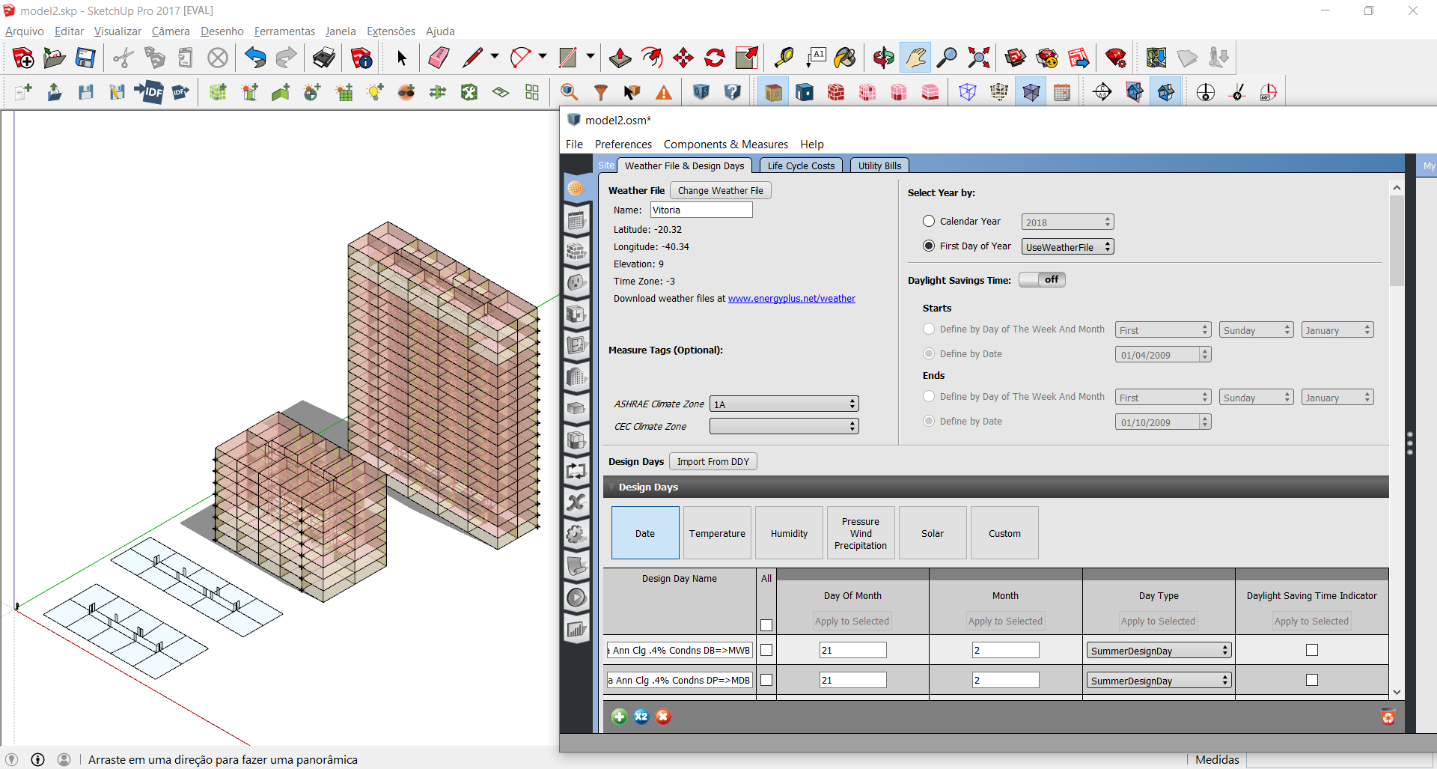
\includegraphics[width=0.8\textwidth]{figures/fig16-OS.png}
    \begin{flushleft}
        \par \small Fonte: autor, (2019).
    \end{flushleft}
    \label{fig:figure16}
\end{figure}
\noindent Concluída a etapa de geometrização e modelagem tridimensional da edificação, é dado início às configurações da envoltória, onde são atribuídos os dados de entrada característicos do empreendimento, como os valores de propriedades térmicas dos elementos construtivos, os dados de ocupação, por meio de schedules para vestimenta, horários de utilização dos ambientes, aberturas, iluminação e equipamentos, como exemplificado na Figura \ref{fig:figure17}.\vspace*{-0.25cm}
\begin{figure}[H]
    \centering
    \caption{Colagem da interface de inserção de dados das propriedades térmicas e de materiais.}
    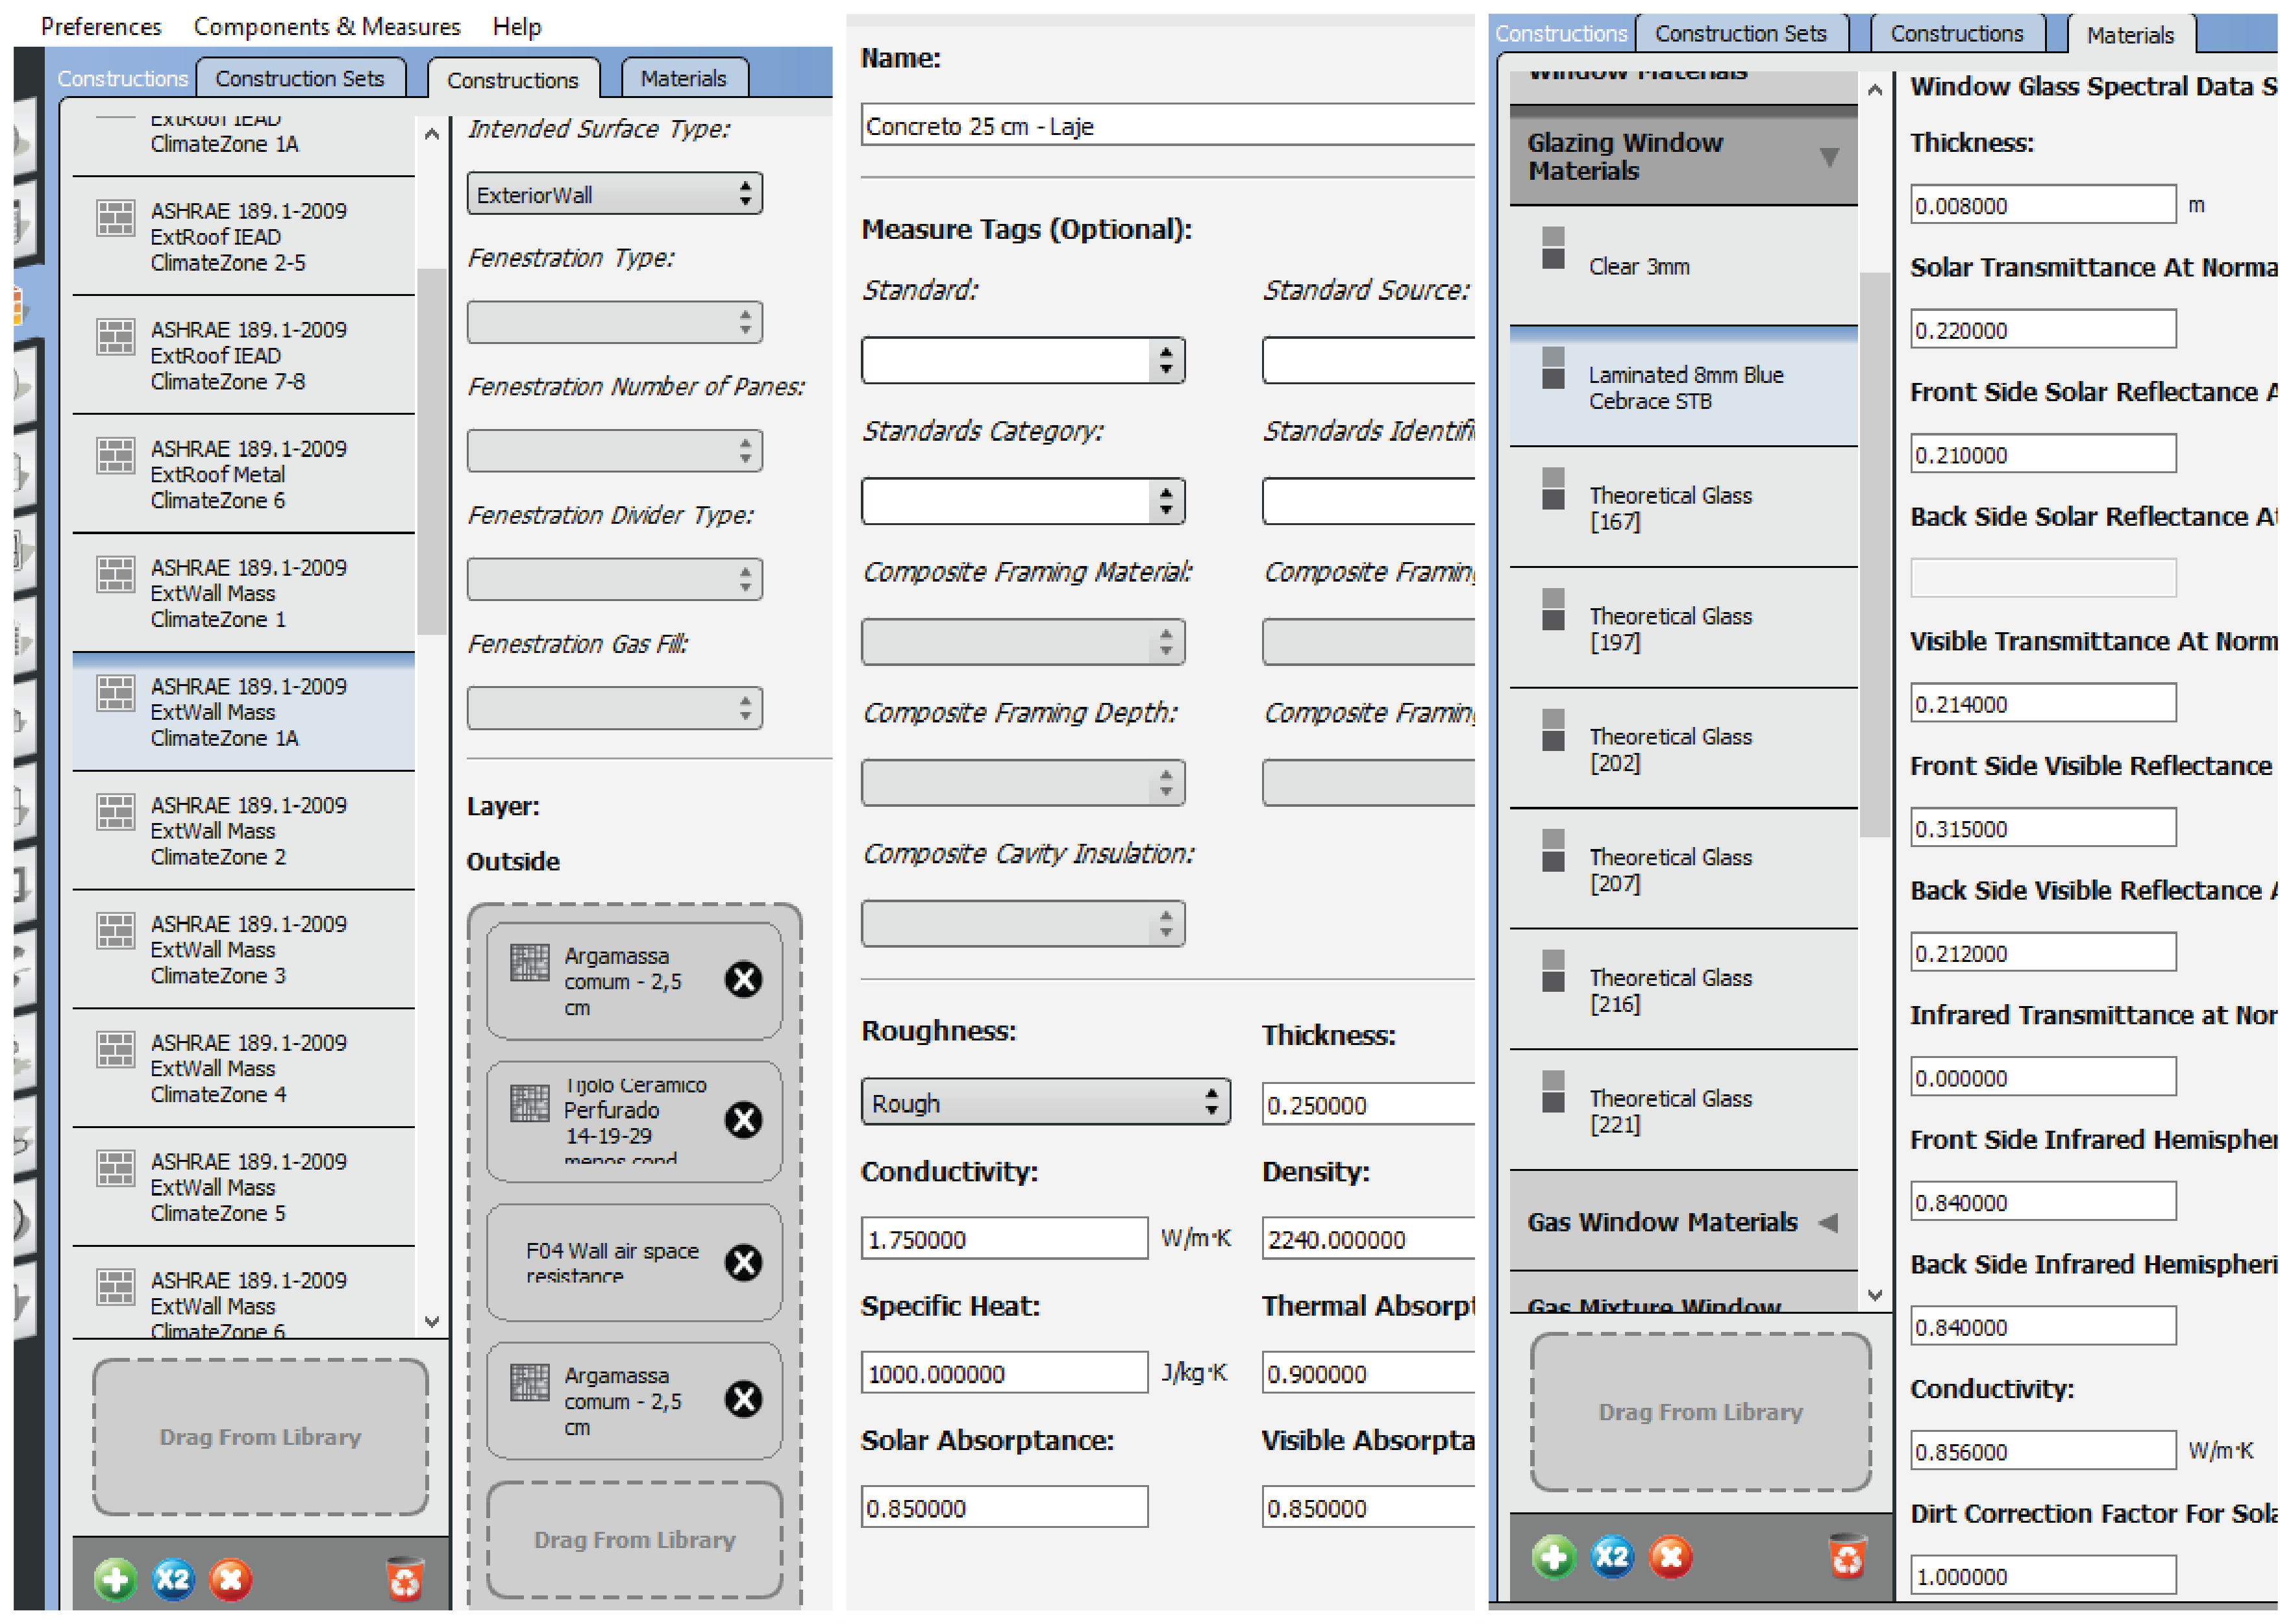
\includegraphics[width=0.8\textwidth]{figures/fig17-OS2.png}
    \begin{flushleft}
        \par \small Fonte: autor, (2019).
    \end{flushleft}
    \label{fig:figure17}
\end{figure}
\noindent Em seguida, foram configurados o sistema de condicionamento de ar, apresentado pela Figura \ref{fig:figure18}, segundo as características definidas para os modelos genéricos. Da mesma forma, foram implementadas medidas de parametrização das variáveis, medidas estas denominadas \textit{measures}, com a finalidade de reduzir o tempo total de processamento e simulação dos cenários. As \textit{measures} adotadas parametrizaram as mudanças de orientação solar, de componentes construtivos, de equipamentos de ar-condicionado e redução de carga de energia.\vspace*{-0.25cm}
\begin{figure}[H]
    \centering
    \caption{Interface de configuração dos sistemas de condicionamento de ar.}
    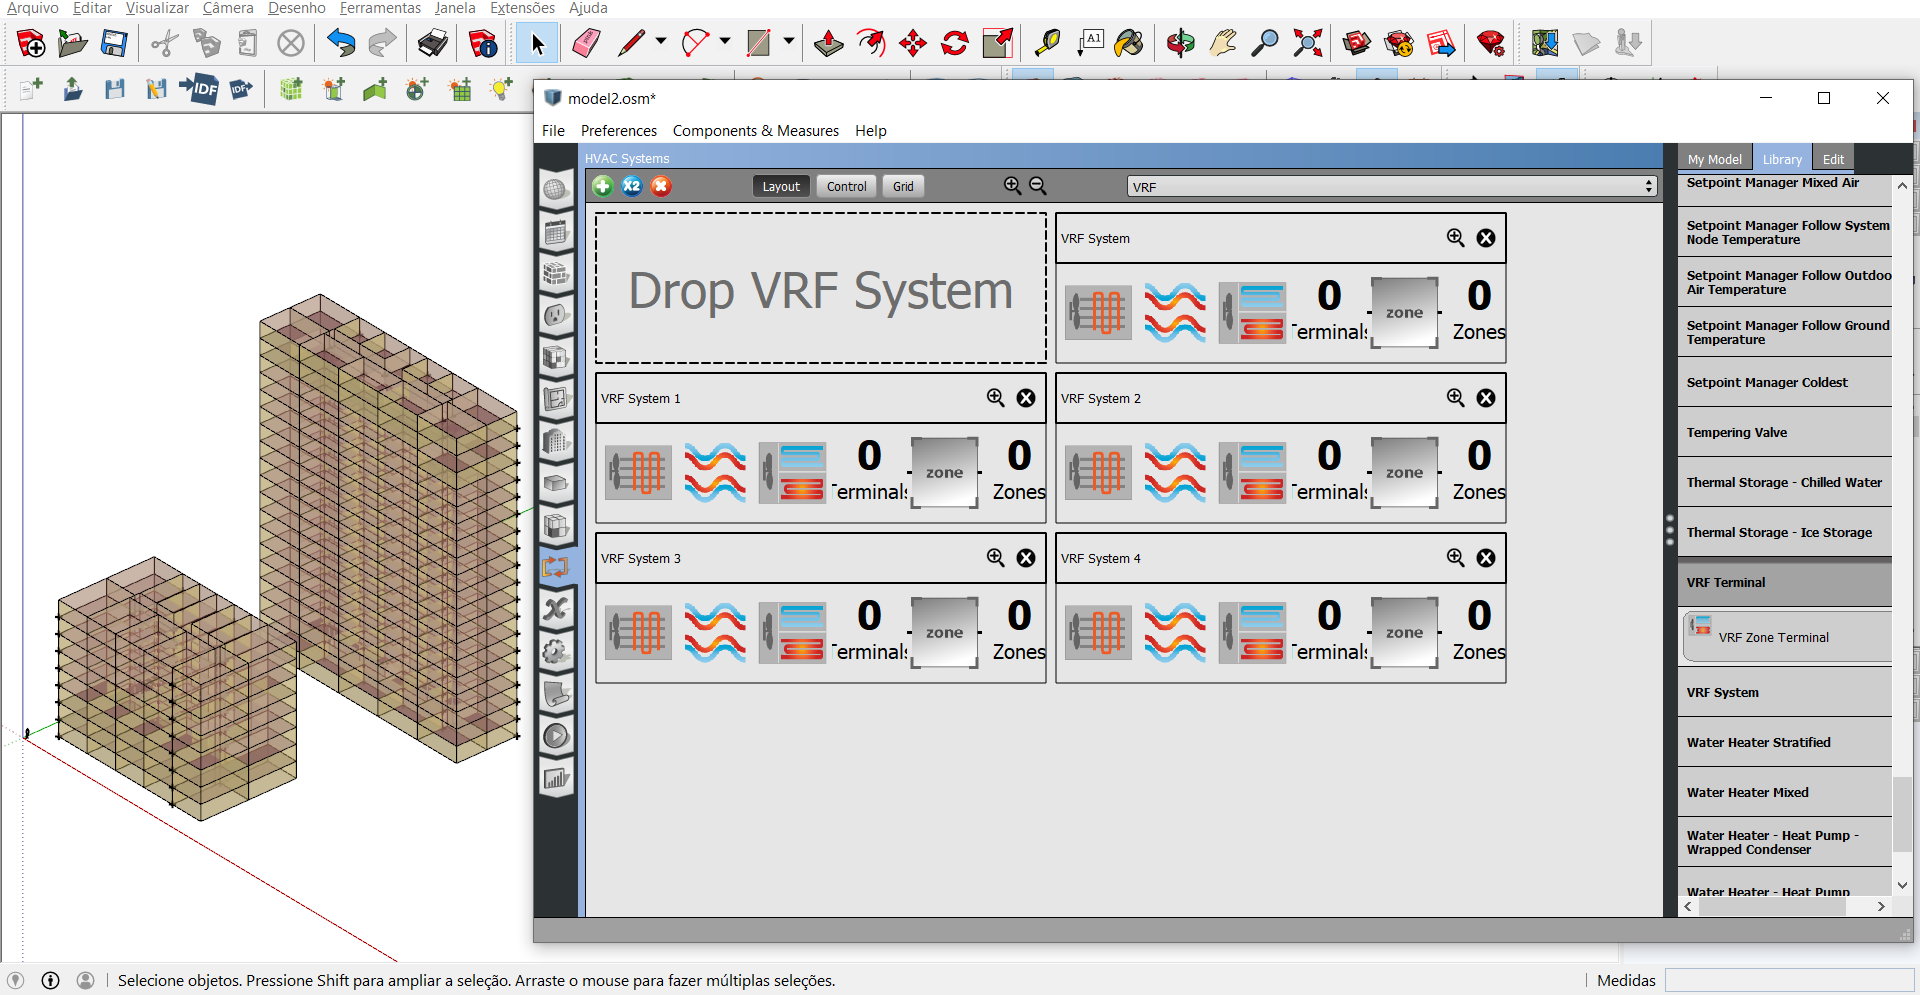
\includegraphics[width=0.85\textwidth]{figures/fig18-OS3.png}
    \begin{flushleft}
        \par \small Fonte: autor, (2019).
    \end{flushleft}
    \label{fig:figure18}
\end{figure}
\noindent Após as configurações de envoltória e sistemas concluídas, foram selecionadas as variáveis de saída relevantes à análise e feito a simulação teste, como exemplificado na Figura \ref{fig:figure19}. Desta forma os resultados foram concentrados nos dados de saída mais pertinentes, reduzindo o tempo total de simulação. Posteriormente, os modelos foram simplificados geometricamente, utilizando o recurso multiply, como abordado no subcapitulo sobre simplificação dos modelos genéricos \cite{Brackney2018}.\newline
\begin{figure}[H]
    \centering
    \caption{Saídas da simulaçãoem processo de finalização.}
    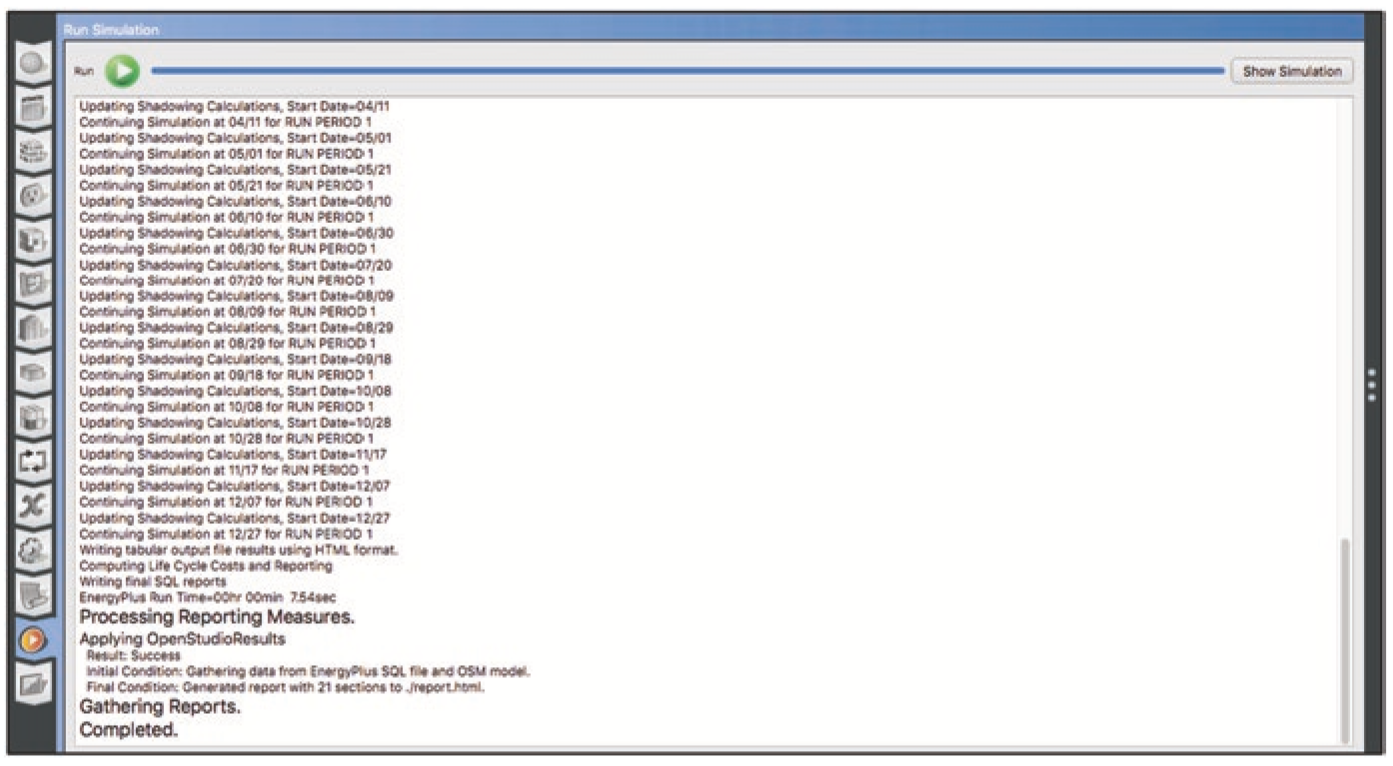
\includegraphics[width=0.9\textwidth]{figures/fig19-OS4.png}
    \begin{flushleft}
        \par \small Fonte: adaptado de Brackney et al. (2018).
    \end{flushleft}
    \label{fig:figure19}
\end{figure}